\section{Evaluations}
\label{sec:eval}

\setlength{\tabcolsep}{1pt}
\begin{table*}[t]
\begin{SmallOut}
\begin{CodeOut}
\begin{center}
\centering \caption {\label{tab:subjects} Characteristics of subjects used in evaluating CAR-Miner.}
\begin {tabular} {|l|c|c|c|c|c|c|c|l|}
\hline
Subject&Lines&\multicolumn{2}{|c|}{Internal Info}&\multicolumn{2}{|c|}{External Info}&\# Code&Time\\
\cline{3-6}
&of code&\#Classes&\#Functions&\#Classes&\#Functions&Examples&(in sec.)\\
\hline
\hline Axion 1.0M2&24k&219&2405&58&217&47783 (7M)&1381\\
\hline HsqlDB 1.7.1&30k&98&1179&80&264&78826 (26M)&2547\\
\hline Hibernate 2.0 b4&39k&452&4321&174&883&88153 (27M)&1125\\
\hline SableCC 2.18.2&22k&183&1551&21&76&47594 (15M)&1220\\
\hline Ptolemy 3.0.2&170k&1505&9617&477&2595&70977 (21M)&1126\\
\hline
\end{tabular}
\end{center}
\end{CodeOut}
\end{SmallOut}\vspace*{-6ex}
\end{table*}

We next describe the evaluation results of CAR-Miner with five
real-world open source applications as subjects. We use the same 
subjects (and same versions) used for 
evaluating a related approach called WN-miner~\cite{WeimerN05}
for the ease of comparison with the data provided by the WN-miner developer.
We used five out of eight subjects used in WN-miner since related versions of the remaining
three subjects are not currently available.
In our evaluations, we try to address the following questions.
(1) Do the exception-handling rules mined by CAR-Miner represent real rules?
(2) Do the detected rule violations represent real defects in subject applications?
(3) Does CAR-Miner perform better than the existing related WN-miner tool in terms of mining real rules and detecting real defects in an application under analysis? 
(4) Do the sequence association rules help detect any new defects that cannot be detected
with simple association rules of the form ``$FC_a$ $\Rightarrow$ $FC_e$''?
The detailed results of our evaluation are available at \url{http://ase.csc.ncsu.edu/projects/carminer/}.
%-------------------------------------------------------------------
\subsection{Subjects}
\label{sec:subjects}

\Comment{Axion is a small and fast open source Java database
engine and provides database management utilities for applications
developed in Java. HsqlDB is one of the leading SQL 
database engines and is often used as a database in development environments. 
Hibernate is a large-scale open source application and is used as a middle ware for interacting
with a database from Java applications. Hibernate allows Java programmers
to develop persistent classes in an object-oriented idiom. SableCC is a parser 
generator that helps build compilers, interpreters, and other text parsers.
Ptolemy is a software framework that studies modeling, simulation, and design
of concurrent, real-time, embedded systems.}
Table~\ref{tab:subjects} shows subjects and their versions used in our evaluations.
Column ``Internal Info'' shows the number of declared classes and functions of each application.
Column ``External Info'' shows the number of external classes and their functions 
invoked by the application. Column ``Code Examples'' shows the number of code examples gathered by CAR-Miner to mine
exception-handling rules. For example, CAR-Miner gathered $47783$ code examples ($\approx$ 7 million LOC) from a code search
engine for mining exception-handling rules of the Axion application. Column ``Time'' shows the amount
of time taken by CAR-Miner in seconds for each application. The shown time includes the analysis time of the
application and gathered code examples, and the time taken for detecting violations.
The amount of processing time depends on the number of samples gathered for an
application. All experiments were conducted on a machine with 3.0GHz Xeon processor and 4GB RAM.

\begin{figure}[t]
\centering
%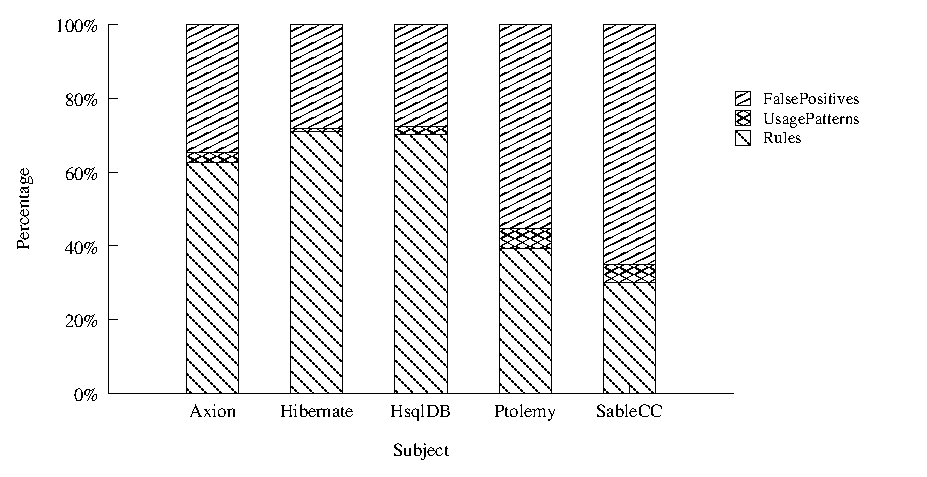
\includegraphics[scale=0.55,clip]{charts/exception-handling-rules.eps}\vspace*{-3ex}
%\caption{\label{chart:exception-handling-rules}Classification of exception-handling rules.}
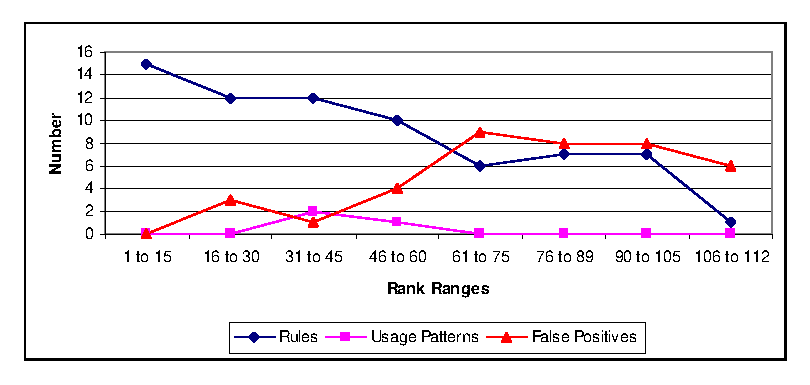
\includegraphics[scale=0.60,clip]{charts/axion-pattern-distribution.eps}\vspace*{-3ex}
\caption{\label{chart:axion-distrib}Distribution of classification categories with ranks for the Axion application.}\vspace*{-5ex}
\end{figure}
%-------------------------------------------------------------------
\subsection{Mined Exception-Handling Rules}
\label{sec:minedrules}

We next address the first question on whether the mined exception-handling rules represent real rules
that can help detect defects in an application under analysis. Table~\ref{tab:minedpatterns} 
shows the classification of exception-handling rules mined by CAR-Miner. Column 
``Total'' shows the total number of rules in each application. 
We classify these rules into three categories: real rules, usage patterns, and false
positives. Real rules describe the behavior that must be satisfied while using function calls
such as $FC_a$, whereas usage patterns suggest common ways of using $FC_a$. The violations of real rules and usage patterns
can be defects and hints, respectively. A hint, which was originally
proposed by Wasylkowski et al.~\cite{wasylkowski07:detecting}, helps increase
readability and maintainability of source code of an application. 
We used the available on-line documentations, JML
specifications\footnote{\url{http://www.eecs.ucf.edu/~leavens/JML/}}, 
or the source code of the application for classifying mined exception-handling rules
into these three categories. Our results show that real rules are  
54.61\% and false positives are 42.16\%, averagely. 
\Comment{The highest number of false positives are found
for the Ptolemy application. The primary reason for a high number of false positives
for Ptolemy is that the exception-handling code include several \CodeIn{get} functions,
which are incorrectly identified as exception-handling rules. In future work, we plan
to address this issue by inlining \CodeIn{get} functions with the associated objects.}

\setlength{\tabcolsep}{1pt}
\begin{table}[t]
\begin{SmallOut}
\begin{CodeOut}
\begin{center}
\centering \caption {\label{tab:minedpatterns}  Classification of exception-handling rules.}
\begin {tabular} {|l|c|c|c|c|c|c|c|c|c|c|}
\hline
Subject&\#Total&\multicolumn{2}{|c|}{Real Rules}&\multicolumn{2}{|c|}{Usage Patterns}&\multicolumn{2}{|c|}{False Positives}\\
\cline{3-8}
&&\#&\%&\#&\%&\#&\%\\
\hline
\hline Axion&112&70&62.5&3&2.68&39&34.82\\
\hline HsqlDB&127&89&70.08&3&2.36&35&27.56\\
\hline Hibernate&121&86&71.07&1&0.82&34&28.09\\
\hline SableCC&40&12&30&2&5&26&65\\
\hline Ptolemy&94&37&39.36&5&5.32&52&55.32\\
\hline \textbf{AVERAGE}&&&54.6&&3.24&&42.16\\
\hline
\end{tabular}
\end{center}
\end{CodeOut}
\end{SmallOut}\vspace*{-4ex}
\end{table}

Although false positives are 42.16\% on average among the total number of mined rules, our mining heuristics
for ranking exception-handling rules help give higher priority to real rules than false positives.
Figure~\ref{chart:axion-distrib} shows a detailed distribution of all extracted rules for the 
Axion application. In Figure~\ref{chart:axion-distrib}, x-axis shows distribution
of mined rules in different ranges (each range is of size 15) with respect to assigned ranks 
and y-axis shows the number of rules that are classified into
the three categories for each range. The primary reason for selecting the Axion 
application is that the application is a medium-scale application that is amenable to a detailed analysis
with reasonable effort. As shown in the figure, the number of false positives is quite low among the 
exception-handling rules ranked between 1 to 60. These results show the significance of 
our mining and ranking criteria. Our results in Table~\ref{tab:minedpatterns} 
also show that more exception-handling
rules exist in applications such as Axion, HsqlDB, and Hibernate that deal with
resources (such as databases or files) compared to other applications. 
%-------------------------------------------------------------------
\setlength{\tabcolsep}{1pt}
\begin{table}[t]
\begin{SmallOut}
\begin{CodeOut}
\begin{center}
\centering \caption {\label{tab:detectedbugs}  Classification of detected violations.}
\begin {tabular} {|l|c|c|c|c|c|}
\hline
Subject&\#Total&\#Violations of&\#Defects&\#Hints&\#FP\\
&Violations&first 10 rules&&&\\
\hline
\hline Axion 1.0M2&257&19&	13 &	1&	5\\
\hline HsqlDB 1.7.1&394& 62&	51 &	0&	10\\
\hline Hibernate 2.0 b4&136& 22	& 12 & 0&	10\\
\hline Sablecc 2.18.2&168& 66	&45 & 7&	14\\
\hline Ptolemy 3.0.2&665& 95	&39	& 1	& 55\\
\hline
\end{tabular}
\end{center}
\end{CodeOut}
\end{SmallOut}\vspace*{-4ex}
\end{table}

\setlength{\tabcolsep}{1pt}
\begin{table}[t]
\begin{SmallOut}
\begin{CodeOut}
\begin{center}
\centering \caption {\label{tab:defectstatus}  Status of detected defects in new versions of subject applications.}
\begin {tabular} {|l|c|c|c|c|c|}
\hline
&\# Defects&New Version&\#Fixed&\#Deleted&\#Open\\
\hline
\hline Axion 1.0M2& 13&	1.0M3&	4&	8&	1\\
\hline HsqlDB 1.7.1& 51&	1.8.0.9&	2&	9&	40\\
\hline Hibernate 2.0 b4& 12	&3.2.6&	0&	8&	4 \\
\hline Sablecc 2.18.2& 45 &	4-alpha.3	&0	&43&	2\\
\hline Ptolemy 3.0.2& 39	&3.0.2	&0	&0	&39\\
\hline
\end{tabular}
\end{center}
\end{CodeOut}
\end{SmallOut}\vspace*{-4ex}
\end{table}
%-------------------------------------------------------------------
\vspace*{-2ex}
\subsection{Detected Violations}
\label{sec:violations}
We next address the question on whether the detected violations represent
real defects. Table~\ref{tab:detectedbugs}
shows the violations detected in each application. Column ``Total Violations''
shows the total number of violations detected in each application. 
The HsqlDB and Hibernate applications include test code as part of their source code.
As test code is often not written according to specifications,
we excluded the violations detected in the test code of those applications 
from the results. Given a high number of violations in each application, we inspected the violations
detected by the top 10 exception-handling rules and classified them into three categories: Defects,
Hints, and False Positives. 

Column ``Violations of first 10 rules'' shows the number of violations
detected by the top ten exception-handling rules mined for each application. 
Column ``Defects'' shows the total number of violations that are identified
as defects in each application. As we used the same versions 
(an earlier version than the latest version)
used by the WN-miner approach for the ease of comparison, 
we verified whether the defects found by our approach are fixed,
deleted, or still open in the latest version of each application. 
Column ``New Version'' of Table~\ref{tab:defectstatus}
shows the latest version used for our verification. 
The defect's sub-categories ``Fixed'' and ``Open'' indicate
that the defects found by our approach in the earlier version are fixed or still open
in the new version, respectively. We reported those open defects to respective
developers for their confirmation. Sometimes, we find that the defective code such as function
body with detected defects does not exist in the latest version.
One reason could be the refactoring of such code, which can be considered 
as an indirect fix. We classified such defects as ``Deleted'' (shown 
in Table~\ref{tab:defectstatus}). 

The results show that our CAR-Miner approach can detect real defects
in the applications. The number of defects shown in Columns ``Fixed''
and ``Deleted'' provide further evidence that these defects detected by CAR-Miner are real
since these defects are fixed directly or indirectly in newer versions of the applications.
The initial response from the developers of HsqlDB is quite
encouraging. The developers responded on the first ten defects that we reported, 
where seven defects are \emph{accepted} and only three defects are rejected.
The bug reports for these ten defects are available in the HsqlDB Bug Tracker
system\footnote{\url{http://sourceforge.net/tracker/?group_id=23316&atid=378131}}
with IDs \#1896449, \#1896448, and \#1896443\footnote{We reported multiple 
defects in the same source file as a single bug report.}.
Although the three rejected defects are 
violations of real rules, developers described that the violation-triggering
conditions of these defects cannot be satisfied in the context of the HsqlDB application.
For example, a rejected defect is a violation of real rule ``\CodeIn{DatabaseMetaData.getPrimaryKeys}
$\Rightarrow$ \CodeIn{ResultSet.close}''. The preceding rule describes
that the \CodeIn{close} function call should be invoked on \CodeIn{ResultSet},
when \CodeIn{getPrimaryKeys} throws any exceptions. The response from the 
developers (Bug report ID: \#1896448) for this defect is 
``\emph{Although it can throw exceptions in general, it should not throw with
HSQLDB. So it is fine.}'', which describes that the violation-triggering
condition cannot be satisfied in the context of HsqlDB.

\Comment{We next describe the real defects detected in Hibernate and HsqlDB
applications, and show how those defects are fixed in the latest version. Figure~\ref{fig:hibernate-fix}
shows a real defect in \CodeIn{Configuration.java} source file (Hibernate 2.0 b4). The defect violated
the exception-handling rule $<$\CodeIn{JarFile.getInputStream}, \CodeIn{JarFile.close}, \CodeIn{null}$>$,
which indicates that when an exception occurs while executing the \CodeIn{getInputStream},
the related \CodeIn{JarFile} resource should be closed. The figure also shows the fix done in the latest
version (version 3.2.6) of the Hibernate application, where a new \CodeIn{finally} block is added
with additional code for closing the \CodeIn{JarFile} resource. A \CodeIn{null} value
in the exception-handling rule indicates that the \emph{trigger} path is empty. The described
defect is not detected by the related approach WN-miner, as this exception-handling rule is extracted
from gathered code examples and does not have supporting samples in the Hibernate application.

\begin{figure*}[t]
\centering
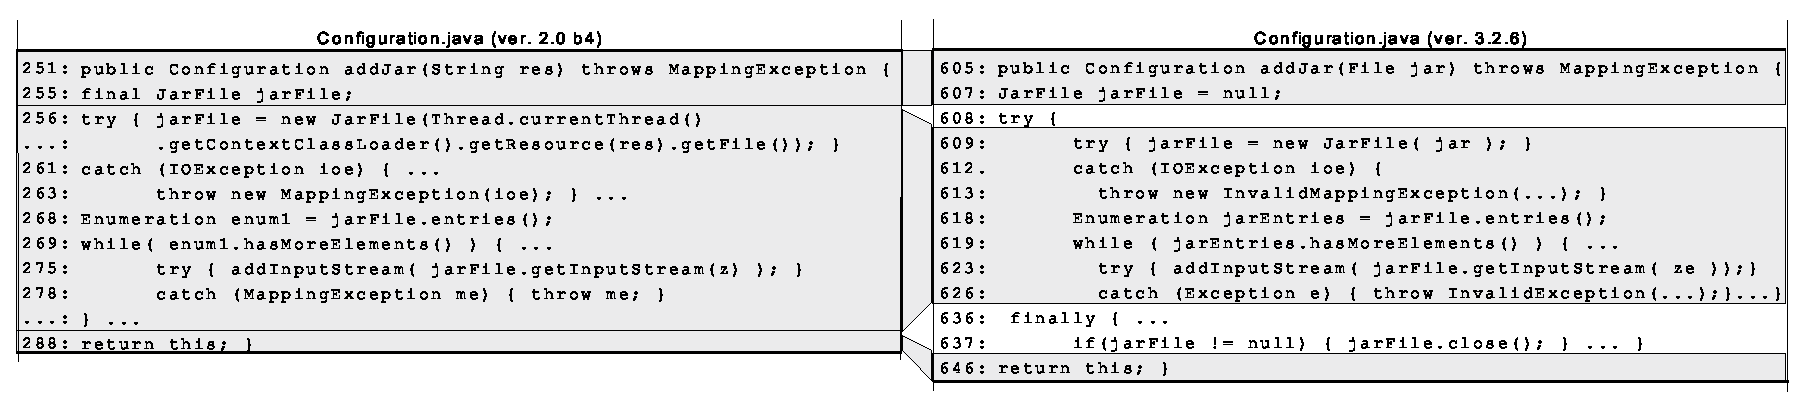
\includegraphics[scale=0.62,clip]{figs/Hibernate-bug-fix1.eps}\vspace*{-2ex}
\caption{\label{fig:hibernate-fix} A fixed defect in the Hibernate application.}\vspace*{-5ex}
\end{figure*}}

%--------------------------------------------------------------------------------------------
\subsection{Comparison with WN-miner}
\vspace*{-2ex}
We next address the third question on whether our CAR-Miner approach performs better than the related 
WN-miner tool. As the WN-miner tool is not currently available, the WN-miner developer provided 
the mined specifications and static traces of their tool. We developed Perl scripts to detect violations
of mined specifications in static traces as described by the WN-Miner developer~\cite{WeimerN05}. 
We used the same criteria described in Sections~\ref{sec:minedrules} and~\ref{sec:violations}
for classifying rules and violations detected by their approach, respectively. 
We compared both mined exception-handling rules and detected violations. 
%---------------------------------------------------------------------------------------------------
\vspace*{-1ex}
\subsubsection{Comparison of exception-handling rules}
\label{sec:comp-weimer-patt}

We next present the comparison results of exception-handling rules mined by both approaches.
Figure~\ref{chart:xweb-wn-pattern} shows the results for the classification category ``real rules'' between WN-miner and CAR-Miner. For each subject and approach, the figure shows the total number of rules mined by each approach
along with the number of common rules between the two approaches. For example,
CAR-Miner detected a total of $70$ rules for the Axion application. Among these $70$ rules,
$43$ rules are newly detected by CAR-Miner and $27$ rules are common between CAR-Miner and WN-miner.
CAR-Miner failed to detect $2$ real rules that were detected by WN-miner. 

\setlength{\tabcolsep}{1pt}
\begin{table}[t]
\begin{SmallOut}
\begin{CodeOut}
\begin{center}
\centering \caption {\label{tab:CAR-Miner-Weimer-defect} Defects detected or missed by CAR-Miner.}
\begin {tabular} {|l|c|c|c|c|}
\hline
Subject&\multicolumn{4}{|c|}{\# Defects}\\
\cline{2-5}
&\# Total&\#Common&\# Only &\# Missed\\
\hline
\hline Axion & 13 & 0 & 13 & 1\\
\hline HsqlDB & 51 & 35 & 16 & 13\\
\hline Hibernate & 12 & 0 & 12 & 7\\
\hline Sablecc & 45 & 0 & 45 & 0\\
\hline Ptolemy & 39 & 38 & 1 & 11\\
\hline \textbf{TOTAL} & 160 & 73 & 87 & 32\\
\hline
\end{tabular}
\end{center}
\end{CodeOut}
\end{SmallOut}\vspace*{-4ex}
\end{table}

The primary reason for these two real rules not detected by CAR-Miner and
detected by WN-miner is due to the \emph{ranking} criterion used by WN-miner. 
WN-miner extracts rules ``$FC_a$ $\Rightarrow$ $FC_e$'' when $FC_e$
appears at least once in exception-handling blocks such as \CodeIn{catch} and ranks those rules
with respect to the number of times $FC_e$ appears after $FC_a$
among normal paths. As shown in their results, such a criterion can result in a high number
of false positives such as ``\CodeIn{Trace.trace} $\Rightarrow$ \CodeIn{Trace.printSystemOut}'' in
the HsqlDB application, where $FC_e$ often appears after $FC_a$ in normal paths and is used
once in some \CodeIn{catch} block. CAR-Miner ignores such patterns due
to their relatively low support among exception paths of $FC_a$.

The results show that CAR-Miner is able to detect most of the rules mined 
by WN-miner and also many new rules that are not detected by WN-miner.
CAR-Miner performed better than WN-miner due to two factors: sequence
association rules and increase in the data scope. To further show the significance
of these factors, we classified the real rules mined by CAR-Miner based
on these two factors. Figure~\ref{chart:trigger-path} shows the percentage of 
sequence association rules among all real rules. The results show that 
sequence association rules are 20.37\% of all real rules on average mined for all applications.

Figure~\ref{chart:data-scope} shows the percentage of real rules 
that cannot be mined by analyzing only the application under analysis. For example,
44.28\% of the real rules mined for the Axion application occur only from 
gathered code samples. Our results show that increase in the data scope
to open source repositories helps detect new exception-handling rules that 
do not have sufficient supporting samples in the application. Furthermore, 
increase in the data scope also helps give higher priority to real rules than false positives.
%------------------------------------------------------------------------------------------
%------------------------------------------------------------------------------------------
\vspace*{-1.5ex}
\subsubsection{Comparison of detected defects}

We next present the number of real defects that were detected by CAR-Miner but not detected by WN-miner. 
To show that CAR-Miner can find new defects that were not detected by WN-miner, we identified
the exception-handling rules that are mined only by CAR-Miner and not by WN-miner
among top 10 shown in Table~\ref{tab:detectedbugs} and verified the defects detected
by those rules. The results are shown in Table~\ref{tab:CAR-Miner-Weimer-defect}.
Column ``Total'' shows the number of violations
detected by the top 10 exception-handling rules. Column ``Common'' and ``Only'' show
the number of defects commonly detected by CAR-Miner and WN-miner, and defects that are detected
by CAR-Miner only, respectively. Column ``Missed'' shows the number of defects
detected by WN-miner only. The results show that CAR-Miner detected $87$ new defects 
(among all applications) that were not detected by WN-miner. 
When inspecting all violations detected by CAR-Miner, we expect that the preceding number
of new defects detected by CAR-Miner can be much higher. 
CAR-Miner missed $32$ defects that were detected by WN-miner. These missed
defects are due to the missing patterns as described in Section~\ref{sec:comp-weimer-patt}.
%------------------------------------------------------------------------------------------
\begin{figure}[t]
\centering
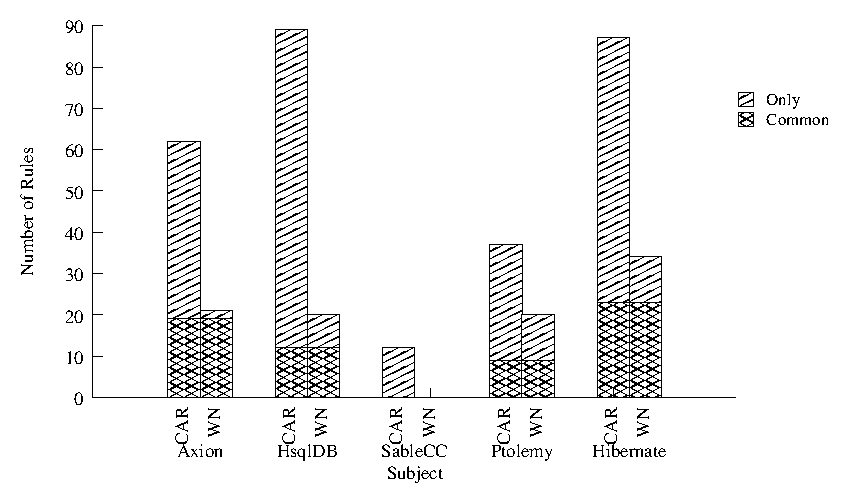
\includegraphics[scale=0.55,clip]{charts/XWeb-Weimer-Patterns.eps}\vspace*{-3ex}
\caption{\label{chart:xweb-wn-pattern}Comparison of real rules mined by CAR-Miner and WN-miner.}\vspace*{-3ex}
\end{figure}
\begin{figure}[t]
\centering
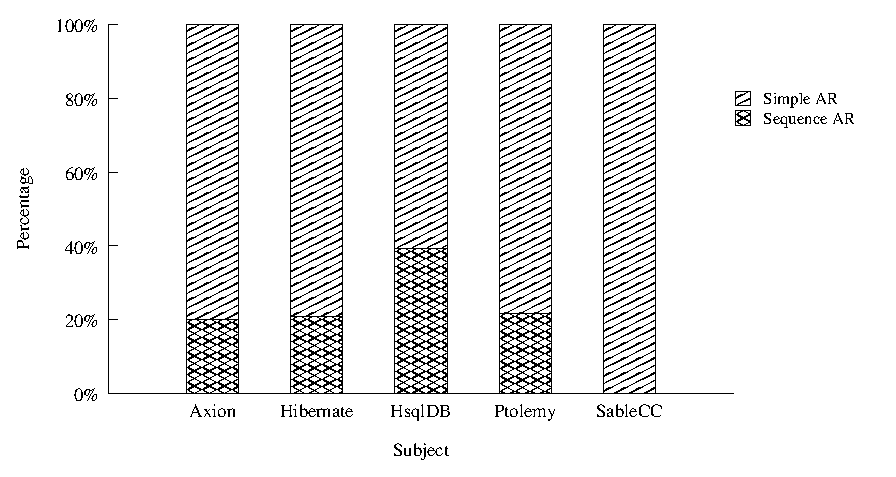
\includegraphics[scale=0.50,clip]{charts/trigger-path.eps}\vspace*{-1ex}
\caption{\label{chart:trigger-path} \% sequence association rules.}
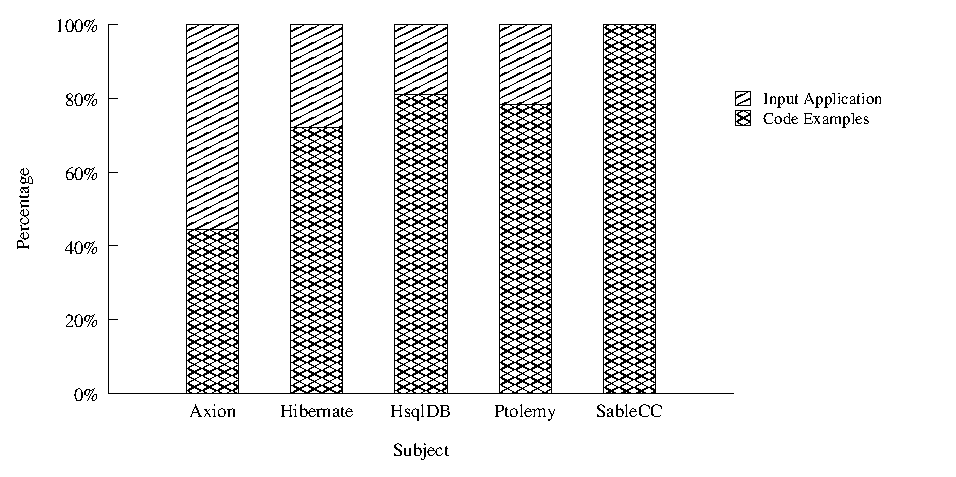
\includegraphics[scale=0.50,clip]{charts/data-scope.eps}\vspace*{-1ex}
\caption{\label{chart:data-scope} \% rules mined only from code examples.}
\vspace*{-3ex}
\end{figure}
%%------------------------------------------------------------------------------------------
\setlength{\tabcolsep}{1pt}
\begin{table}[t]
\begin{SmallOut}
\begin{CodeOut}
\begin{center}
\centering \caption {\label{tab:condassorules} Defects detected by Sequence Association Rules.}
\begin {tabular} {|l|c|c|c|c|c|}
\hline
&\# Rules&\# Violations&\# Defects&\# Hints&\# False Positives \\
\hline
\hline Axion & 3 & 6 & 4 & 0 & 2\\
\hline HsqlDB & 6	& 14	&8	&0	&6\\
\hline Hibernate & 4 &10	&8	&0	&2\\
\hline Sablecc & 0 &0	&0	&0	&0\\
\hline Ptolemy & 1 &1	&1	&0	&0\\
\hline
\end{tabular}
\end{center}
\end{CodeOut}
\end{SmallOut}\vspace*{-6ex}
\end{table}
%%------------------------------------------------------------------------------------------
\subsection{Significance of Sequence Association Rules}
\vspace*{-2ex}
We next address the last research question on whether sequence association rules 
mined by CAR-Miner are helpful in detecting new defects that cannot be detected
by simple association rules. Table~\ref{tab:condassorules}
shows the number of sequence association rules that are used to detect real defects
in all applications. The results show that these rules help detect $21$ real defects among
all applications. 

We next describe a defect in the HsqlDB application to show the significance
of sequence association rules, which cannot be mined by existing approaches such as WN-miner.
The related code snippet from the \CodeIn{saveChanges} function of \CodeIn{ZaurusTableForm.java} is shown as 
below:
\vspace*{-1ex}
\begin{CodeOut}
\begin{alltt}
public boolean saveChanges() 
\{ ...
\hspace*{0.1in}try \{ 
\hspace*{0.2in}PreparedStatement ps = 
\hspace*{0.5in}cConn.prepareStatement(str);
\hspace*{0.2in}ps.clearParameters(); ...
\hspace*{0.2in}for (int j=0; j<primaryKeys.length; j++)\{
\hspace*{0.3in}ps.setObject(i + j + 1, 
\hspace*{0.5in}resultRowPKs[aktRowNr][j]); \}
\hspace*{0.2in}ps.executeUpdate();
\hspace*{0.1in}\} catch (SQLException e) \{ ...
\hspace*{0.3in}return false; 
\hspace*{0.1in}\} ...
\}
\end{alltt}
\end{CodeOut}
\vspace*{-1ex}
CAR-Miner detected a defect in the preceding code example as the code example violated the exception-handling rule
$FC_c^1$ $\wedge$ $FC_a$ $\Rightarrow$ $FC_e^1$, where

$FC_c^1$:\CodeIn{Connection.prepareStatement}\\
\hspace*{0.15in}$FC_a$ :\CodeIn{PreparedStatement.clearParameters}\\
\hspace*{0.15in}$FC_e^1$ :\CodeIn{Connection.rollback}\\
\vspace*{-1ex}

The preceding rule describes that when an exception occurs after executing the \CodeIn{clearParameters} function, the \CodeIn{rollback} function should be invoked on the \CodeIn{Connection} object. Failing to invoke 
\CodeIn{rollback} can make the database state inconsistent. This result shows that sequence
association rules are helpful in detecting new defects.